\documentclass[border=8pt]{standalone}
\usepackage[utf8]{inputenc}
\usepackage[romanian]{babel}
\usepackage{tikz}
\usetikzlibrary{arrows.meta,decorations.pathreplacing,calc}

\begin{document}
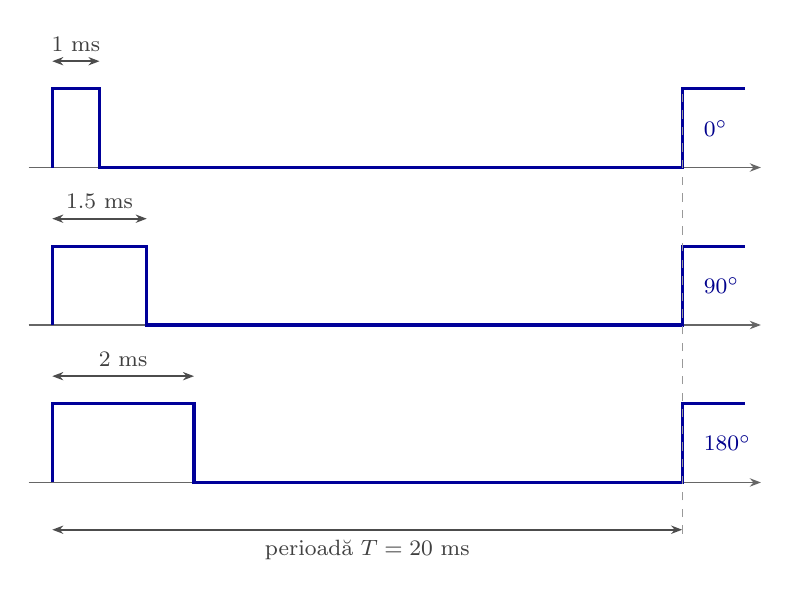
\begin{tikzpicture}[
  font=\small,
  >={Stealth[length=4pt]},
  sig/.style={line width=1.1pt},
  ax/.style={->,line width=0.7pt,black!60},
  dimn/.style={<->,line width=0.6pt,black!70},
  lab/.style={font=\footnotesize,text=black!75}
]

% parametri de desen (nu la scara reala: pulsul e largit ca sa se vada)
\def\T{8}        % o perioada in unitati de desen (= 20 ms)
\def\H{1.0}      % inaltimea pulsului
\def\dy{2.0}     % spatiu vertical intre forme de unda

% --- macro pentru o forma de unda PWM cu latime de puls p (in unitati desen) ---
% #1 = y de baza, #2 = latime puls, #3 = eticheta puls, #4 = eticheta unghi
\newcommand{\pwmrow}[4]{
  \draw[ax] (-0.3,#1) -- (\T+1.0,#1);                 % axa timp
  \draw[sig,blue!60!black]
     (0,#1) -- (0,#1+\H) -- (#2,#1+\H) -- (#2,#1)
     -- (\T,#1) -- (\T,#1+\H) -- (\T+0.8,#1+\H);       % puls + start perioada urmatoare
  % cota latime puls
  \draw[dimn] (0,#1+\H+0.35) -- (#2,#1+\H+0.35)
     node[midway,above,lab]{#3};
  % eticheta unghi (dreapta)
  \node[lab,anchor=west,text=blue!55!black] at (\T+0.15,#1+\H/2) {#4};
}

% trei cazuri
\pwmrow{2*\dy}{0.6}{1~ms}{$0^\circ$}
\pwmrow{1*\dy}{1.2}{1.5~ms}{$90^\circ$}
\pwmrow{0}{1.8}{2~ms}{$180^\circ$}

% cota perioada (sub forma de jos)
\draw[dimn] (0,-0.6) -- (\T,-0.6) node[midway,below,lab]{perioadă $T = 20$~ms};
\draw[black!40,dashed,line width=0.5pt] (\T,-0.65) -- (\T,2*\dy+\H);

\end{tikzpicture}
\end{document}
